\section{Background: Serverless Computing}\label{sec:background}

%To address the characteristics of edge computing nodes, an edge platform must manage its resources very efficiently, which means provisioning and allocating resources only when they are needed. 

%data size as a criteria for the offloading decision
\begin{figure*}[tbp]
	\centering
	\captionsetup[subfigure]{width=0.48\linewidth}
	\subfloat[Both \textit{feature extraction} and \textit{matching} compose a single service (fEM); mobile devices (md) are unable to offload computation to SEP A, whose resources have been allocated to other functions; computation is offloaded to SEP B with one \textit{HTTP request} per video frame.\label{fig:Mobile_Computation_Offloading_F1}] {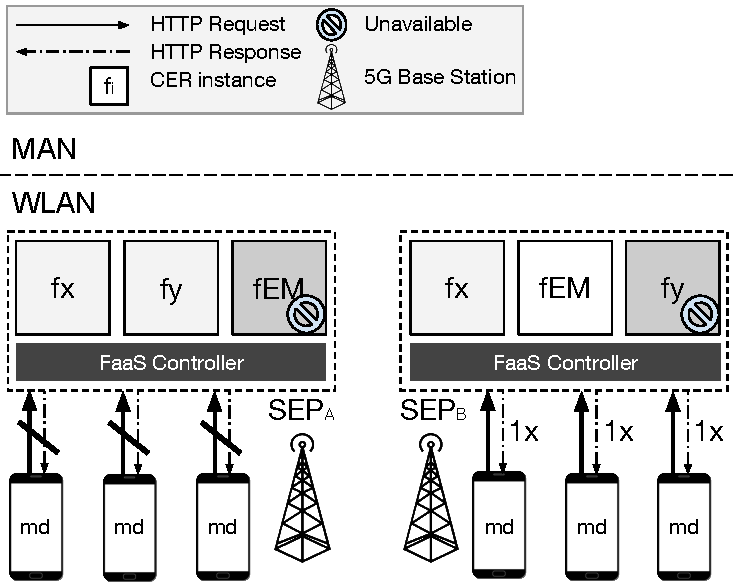
\includegraphics[width=0.48\textwidth]{Figs/Mobile_Computation_Offloading_F1.pdf}}
	~
	\captionsetup[subfigure]{width=0.51\linewidth}
	\subfloat[Data-intensive \textit{feature extraction} (fE) is performed by SEP A and B; whereas \textit{feature matching} (fM) is offloaded from SEP A to SEP B or to a Regional SEP by a \textit{Load Balancer}. In total, computation is offloaded to either SEP with two \textit{HTTP requests} per video frame.\label{fig:Mobile_Computation_Offloading_F2}] {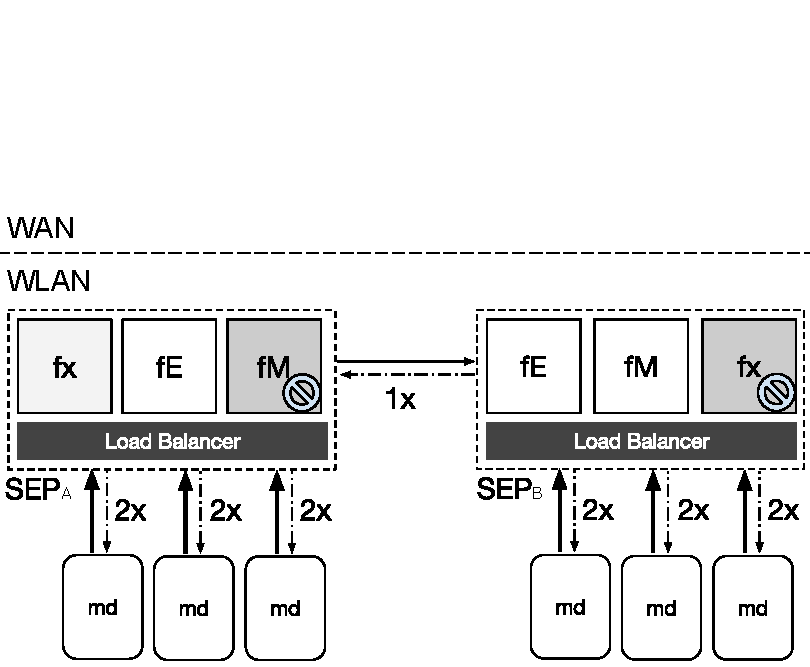
\includegraphics[width=0.51\textwidth]{Figs/Mobile_Computation_Offloading_F2.pdf}}
	\caption{\textit{Feature extraction} and \textit{matching} functions from the AR example forming a single (a), and two fine-grained services (b)} \label{fig:Mobile_Computation_Offloading}
\end{figure*}

Serverless computing~\cite{Lloyd18serverless,Roberts:2018} is mainly associated with two concepts: of applications that rely on third-party cloud services for handling business logic and state (also known as background-as-a-service, or BaaS); and that of applications for which server-side logic is still written by application developers, but, unlike traditional architectures, runs in stateless compute containers that are event-triggered
%, ephemeral (may only last for one invocation), 
and fully managed by a third party (also known as functions-as-a-service, or FaaS).

In the FaaS model, application logic is implemented as functions, which may be written in various languages and exposed as web services. Functions are packed along with its dependencies (e.g., modules, libraries, other resources); runtime instances (e.g., NodeJS, Python) are made available on demand within milliseconds, thanks to the container technology. Functions can be executed just once, frequently, or concurrently. After completion, containerized runtime instances may remain idle (warm) for a short period of time before been reused or released.

If compared to the conventional Infrastructure-a-as-Service model (IaaS), the FaaS model ensures resources to be allocated when actually needed. FaaS platforms (e.g., AWS Lambda~\cite{AWSLambda}) also enforce limitations to the function package size and execution time by design. Due to its characteristics, this execution model enables an efficient usage of shared computational resources, which is particularly important to cope with the resource limitations of edge platforms and to allow edge-based solutions to scale~\cite{GarrigaMendonca2017}.



%The achieve efficiency is particularly important in the context of fine-grained edge nodes exhibiting limited computational and storage resources. 

%a higher number of concurring functions~\cite{}.

%

%Also, users are billed by the actual usage of resources (pay-as-you-go). This model may give edge infrastructure providers a .

%\subsection{Edge Infrastructure and Architecture}

%Regardless of...